%V ďalšej časti prezentujte vlastný prínos a vlastné výsledky porovnajte s výsledkami iných. Charakterizujte použité metódy.
%Vyhýbajte sa používaniu žargónu.
%Používajte starú múdrosť: 1 obrázok je viac než 1000 slov.

\subsection{Analysis} 
In this section we present in--depth analysis of the Two learning rate model.  

\subsubsection{Performance} 

TODO Explain how it was measured (runs, epochs, stopping) \\
TODO Explain / Make up hypotheses why it behaves as measured (Future work). \\

%TODO treat as main plot of the work 
%TODO (add plane of best BAL) 
\begin{figure}[t]
  \centering
  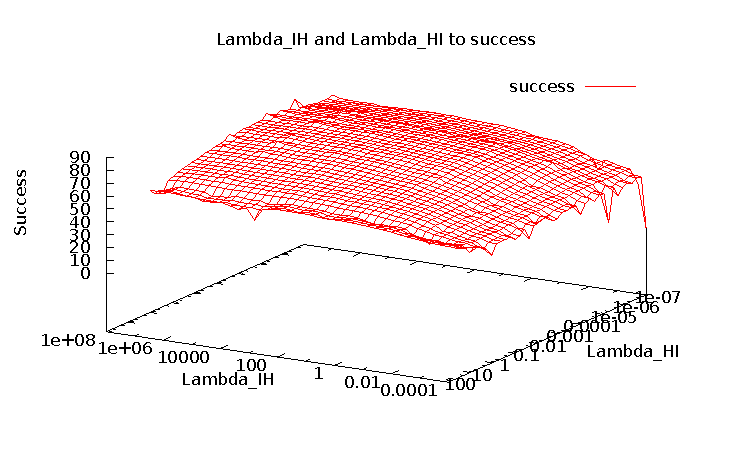
\includegraphics[width=0.8\textwidth]{img/success_to_lambdas.pdf}    
  \caption{Encoder 4-2-4: Performance of the TLR model with $\sigma = 2.3$ and $\mu = 0.0$.}
  \label{fig:results-two-lambdas-auto4-success}
\end{figure}

%TODO logaritmic scale of epochs + label 
\begin{figure}[t]
  \centering
  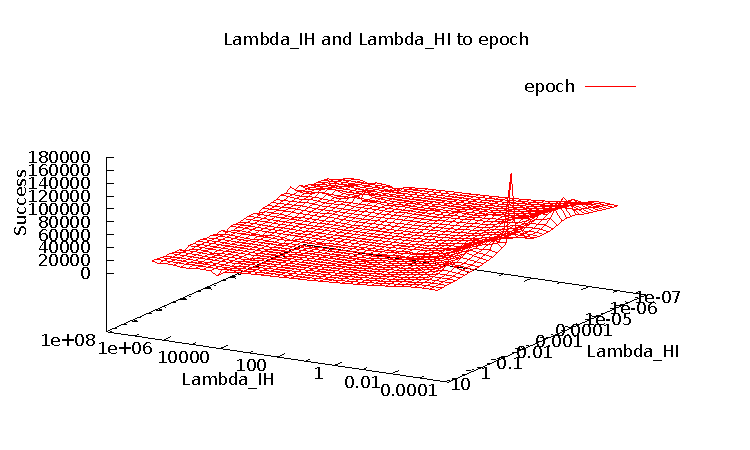
\includegraphics[width=0.8\textwidth]{img/epoch_to_lambdas.pdf}    
  \caption{Encoder 4-2-4: Convergence time of the TLR with $\sigma = 2.3$ and $\mu = 0.0$.}
  \label{fig:results-two-lambdas-auto4-epoch}
\end{figure}

% TODO bitSucc, patSucc, F,B + std_dev 
\begin{figure}[t]
  \centering
  \includegraphics[width=0.8\textwidth]{../bal/data/stats/test/epoch_to_success.pdf}    
  \caption{Encoder 4-2-4: Epoch to success of the best Two learning rate setting for $\lambda_v = $ and $\lambda_h=$ (TODO values).}
  \label{fig:results-two-lambdas-auto4-s2e} 
\end{figure}

\subsubsection{Important features}
\label{sec:results-candidates} 

With the candidate selection experiment \ref{sec:our-candidates} we have found the most important features. 

\begin{figure}[h]
  \centering
  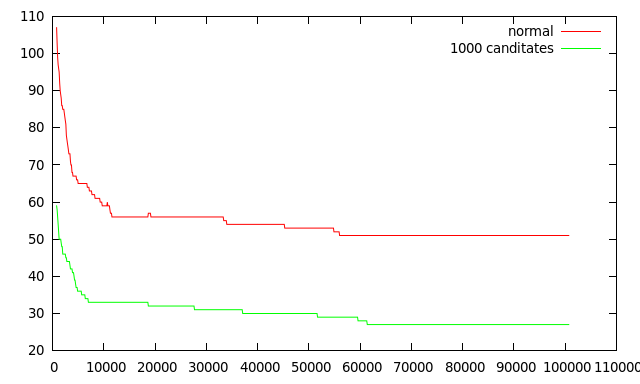
\includegraphics[width=0.8\textwidth]{../presentation/img/long_run_error.png}    
  \caption{Encoder 4-2-4 - Candidate selection vs. normal BAL}
  \label{fig:TODO-4}
\end{figure}

TODO Hidden distance (over 70\%); in triangle (68.3 \%). 

\begin{figure}[h]
  \centering
  \includegraphics[width=0.8\textwidth]{../bal/data/stats/test/epoch_to_h_dist.pdf}    
  \caption{Encoder 4-2-4: The following figure shows that when selecting the candidate with the highest \emph{h\_dist} among 1000 randomly generated networks it could lead to $\approx 10\%$ success increase. }
  \label{fig:TODO-2}
\end{figure}


TODO Linear regression model. 

\subsubsection{Observations}
\label{sec:results-two-lambdas}  %TODO (still relevant label? ) 

Other partial results we found interesting. 
TODO talk about these points (item -> paragraph ; item -> other results): 

\begin{itemize} 
\item TODO! momentum 0.01 seems to add to performance / convergence 
\item Matrices IH-OH and HO-HI tend to be same in autoassociative tasks. 
\item Hidden representation distance is a meaningful measure (LinReg on pre\_measure) (+ 10\%) . 
\item In triangle (non-convex). Not-in triangle is a must to condition for success. \\
TODO rerun to get "1 err in\_triangle" with and without preselection (there was a bug in the old data). 
\item Long run (+ 10\%). It seems it's always better to have long runs. even after 800,000 epochs there are some networks for which the error change
\item reprezentacie na hidden absolutne rovnake (forward, backward), matice rozne:
\item Convergence Epsilon - weights tend to infinity (09-12-2013: Convergence which depends on average weight change does not work). 
\item Rerun - same config, different order when training 
All bad: \\
err sigma lambda momentum success sample\_ratio \\
0.0 2.3 0.7 0.0 19.296918767507005 6889/35700 \\
1.0 2.3 0.7 0.0 68.05602240896359 24296/35700 \\
2.0 2.3 0.7 0.0 12.644257703081232 4514/35700 \\
3.0 2.3 0.7 0.0 0.0028011204481792717 1/35700 \\

All good:  \\
err sigma lambda momentum success sample\_ratio \\
0.0 2.3 0.7 0.0 99.98911353032659 64293/64300 \\
1.0 2.3 0.7 0.0 0.01088646967340591 7/64300 \\
\end{itemize}




